\documentclass{jcst}

% The JCS&T template requires the following packages installed in your LaTeX2 distribution:
% etoolbox,flushend,microtype,lmodern,sectsty,graphicx,booktabs,geometry,amssymb,amsmath,amsthm,
% authblk,mathptmx, babel


\title{Author's Guide for Preparing a Paper for the Journal of Computer Science \& Technology \\
\large Gu\'{i}a para Autores que Preparen un Art\'{i}culo para Journal of Computer Science \& Technology}

\author[1,2\orcid{0000-0002-1825-0097}]{First Author}
\author[2\orcid{0000-0002-1825-0097}]{Second Author}
\author[1\orcid{0000-0002-1825-0097}]{Last Author}

\affil[1]{University Department, University Name, Country \authorcr
\{firstauthor, lastauthor\}@mail.dom }
\affil[2]{Group, Company, Country  \authorcr
secondauthor@mail.dom}



\begin{document}

\maketitle

\begin{abstract}
These instructions give you guidelines for preparing papers for the Journal of Computer Science \& Technology. The abstract should summarize the  content of the paper. The abstract should be below 200 words. Do not make references nor display equations in the abstract. The journal will be printed   by photo-offset from the same-sized copy prepared by you. Your manuscript should be printed on A4 paper (21.0 cm x 29.7 cm). It is imperative that the margins and style described below be adhered to carefully. This will enable us to keep uniformity in the final printed copies of the Journal. Please
 keep in mind that the manuscript you prepare will be printed practically as it is received.  Readability of copy is of paramount importance.
\end{abstract}

\keywords{Enter key words or phrases in alphabetical order (5 maximum), separated by commas.}

\renewcommand{\abstractname}{Resumen}
\begin{abstract}
This section should be a properly Spanish translated version of the Abstract. The limit of 200 words remains as in the previous section.
\end{abstract}

\palabrasclaves{Enter previous key words or phrases in alphabetical order in Spanish, separated by commas.}


\section{Important Information}

The submitted papers must be original. Do not submit a reworked version of a paper you
have submitted or published elsewhere. Do not publish preliminary data or results.
The submitting author is responsible for obtaining agreement of all coauthors and
any consent required from sponsors before submitting a paper. The authors must
 cite relevant prior work.
There is a limit of 15 pages for each paper in the Journal, but authors can ask for additional pages (if required). Each submission should
be a .pdf file submitted through the JCS\&T management system.


\section{Preparation of Manuscript}

\subsection{General Appearance}

The text must be in English but title, abstract and keywords must be included in Spanish too. The submitted typeset scripts of each contribution must be in their final form and of good appearance since they will be printed with minor edition. It is essential that the \textit{camera-ready copies} be absolutely clean.

Your paper must be printed in two columns. Columns should be balanced in the last page. The document you are reading is printed in the format that should be used in your paper.

\subsection{Specification}

To ensure uniformity of appearance for the Journal, your paper should conform to
 the following specifications. If your paper deviates from these
 specifications, the printer may not be able to include your paper in the Journal.

\begin{enumerate}
\item The top, bottom, left, and right margins should be 2.5 cm, except for the first page where the top margin should be 3.5 cm.
\item The distance between the two columns of text should be 1cm.
\end{enumerate}

\section{Font size}
The font size must be 10 points. This document is set in 10-point. Some technical
formatting programs print mathematical formulas in italic type, with subscripts
and superscripts in a slightly smaller or bigger font size. This is acceptable.

\section{Major Headings}

Major headings are to be left-aligned, in a bold font without underline and
must be numbered. For example, the text
 \textbf{4. Major headings} at the top of this paragraph is a major heading.

\subsection{Subheadings}
Subheadings should be in a bold font and start at the left-hand margin on a separate line.

\subsubsection{Sub-subheadings}
Sub-subheadings should be in a bold font and left-aligned too.

\section{Figures}

The figures can be in color. However, because printed version will be in
 black and white, you must ensure a clear view in grayscale. All figures must be in PNG or EPS format, having at least 200 DPI. The caption must be placed \textit{after} the
 graphic. All figures must be mentioned in text, like this Fig.~\ref{fig:sampleimage-sc}.

\begin{figure}[ht]
\centering
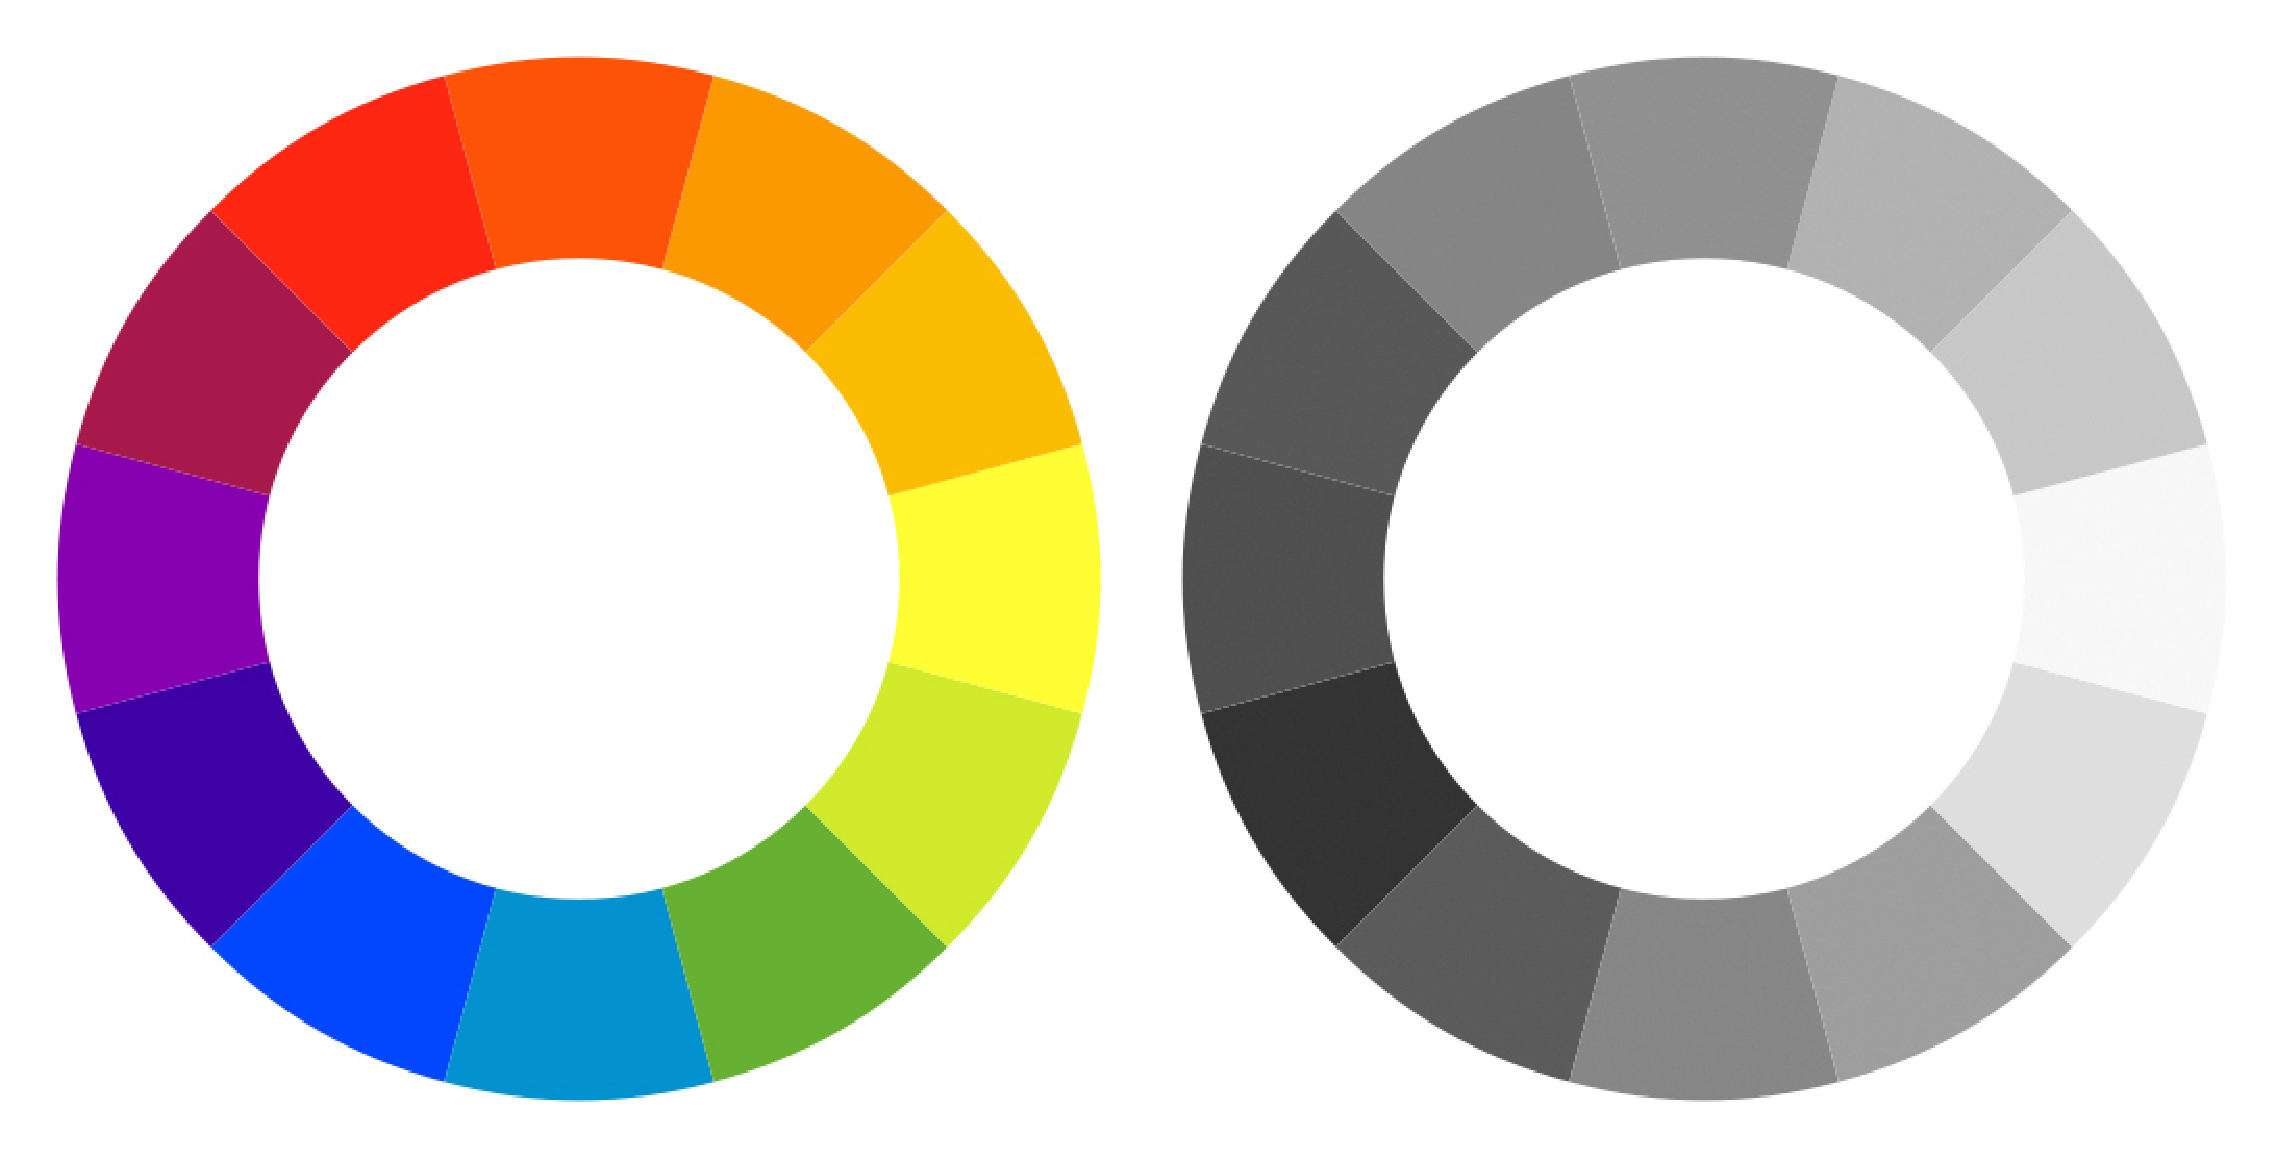
\includegraphics[width=0.4\textwidth]{colors}
\caption{\label{fig:sampleimage-sc}Sample image in single-column format}
\end{figure}

A figure can appear in double-column format (if convenient), as Fig.~\ref{fig:sampleimage-dc}. 

\begin{figure*}[t]
\centering
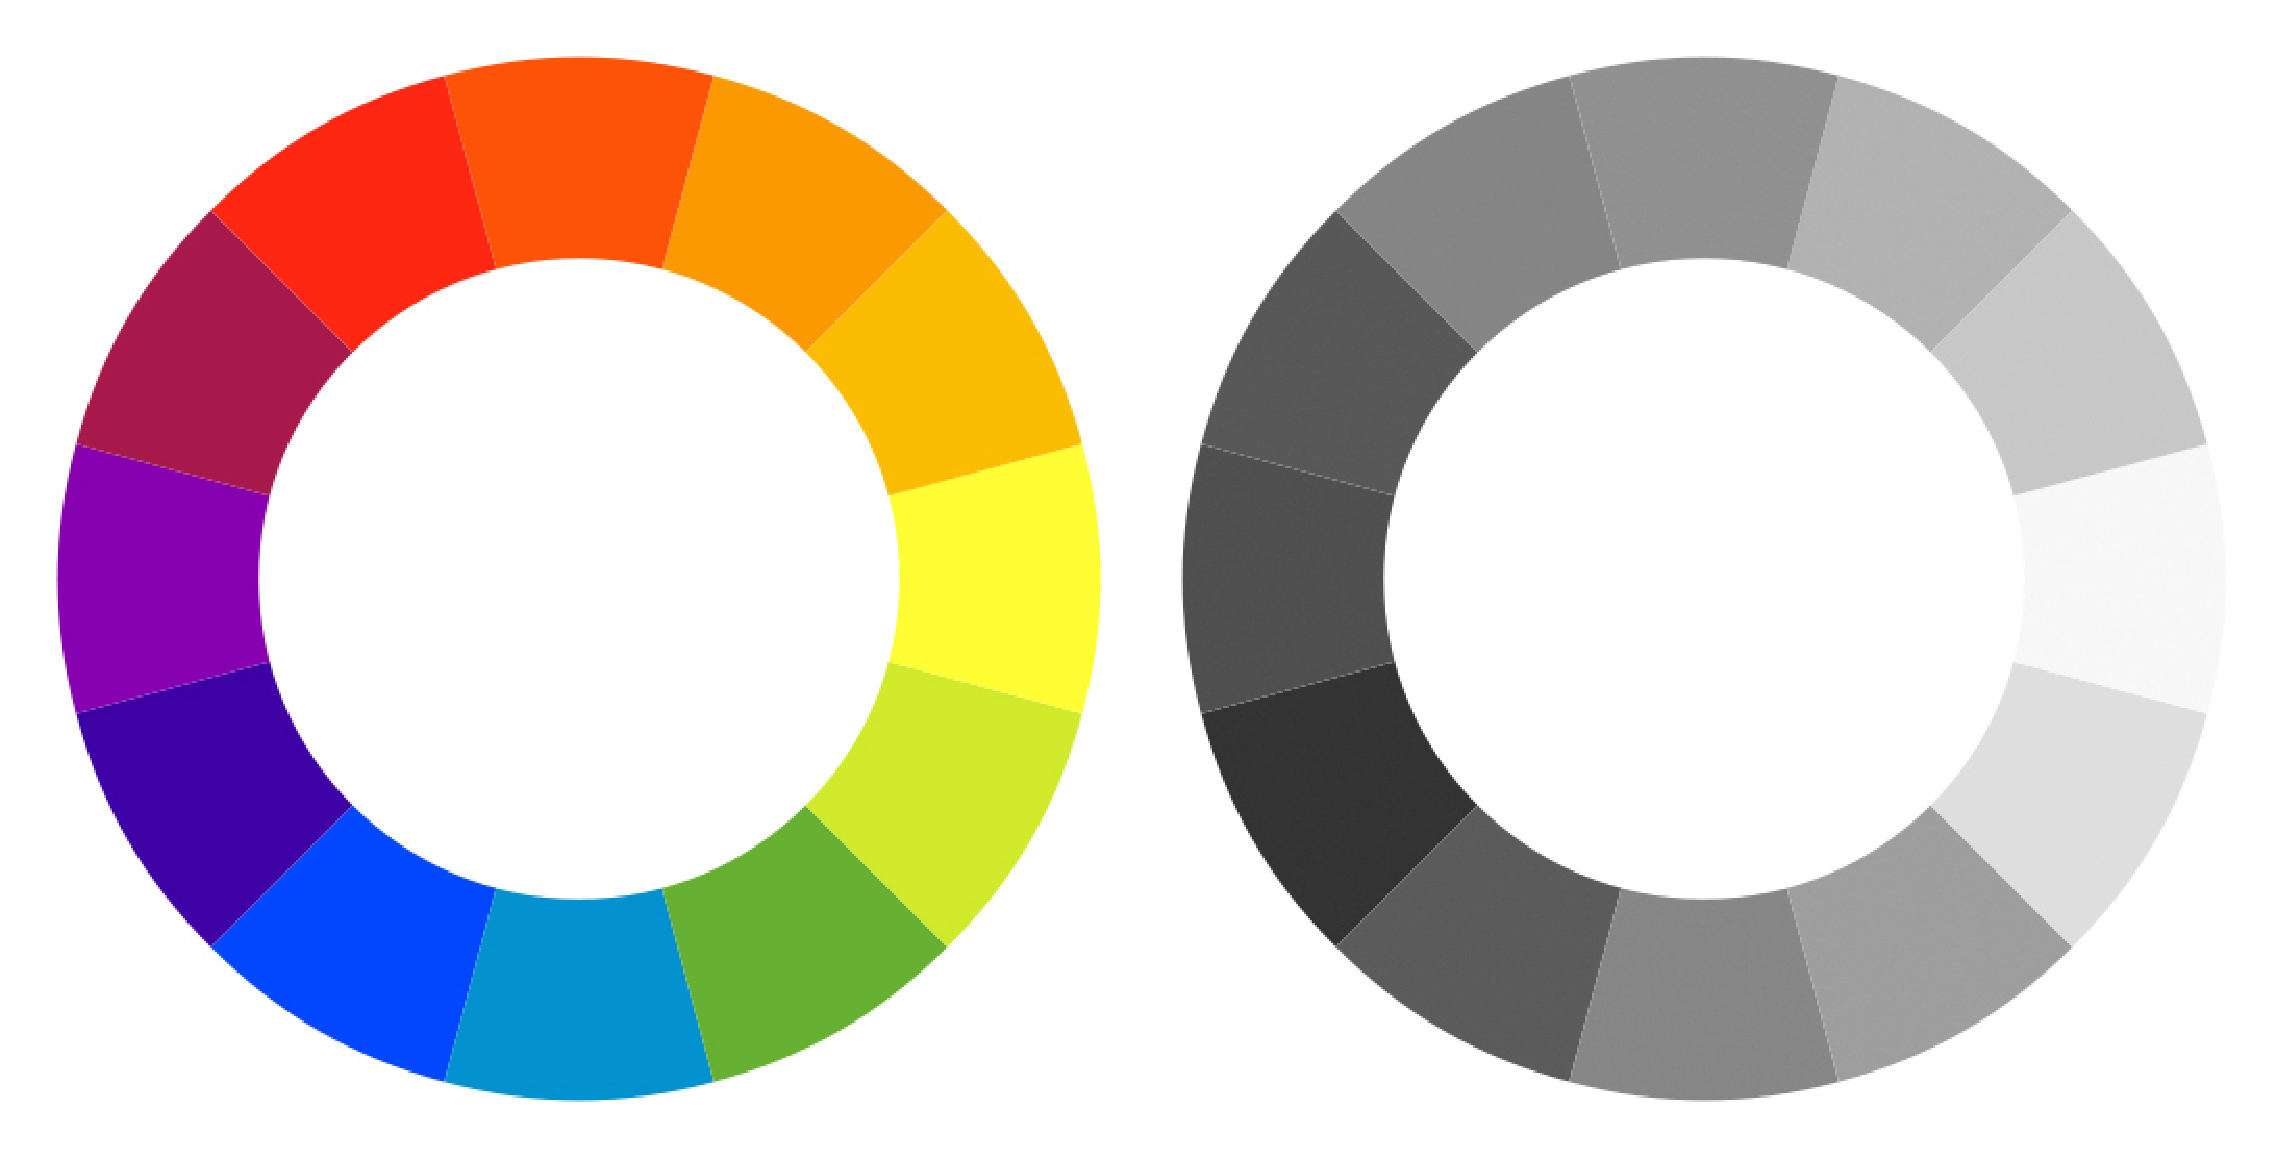
\includegraphics[width=0.6\textwidth]{colors}
\caption{\label{fig:sampleimage-dc}Sample image in double-column format}
\end{figure*}

\section{Algorithms}

Algorithms must be in black and white. The caption must be placed before the algorithm and is obligatory. All algorithms must be mentioned in text, like this Algorithm~\ref{alg:samplealg}.

\begin{algorithm}[ht]
\caption{Sample algorithm}\label{alg:samplealg}
	\begin{algorithmic}[1]
		\State {$sum = 0$}		\Comment{Initialize $sum$}
		\For{$i \leq n$} 
			\If{$i \% 2 == 0$}
	       		\State{$sum += i$}
	       	\EndIf
		\EndFor
		\State{print($sum$)} 
	\end{algorithmic}
\end{algorithm}


\section{Equations}
All equations must be typed in black. They should be numbered
consecutively throughout the text. Equation numbers should be enclosed in
parentheses and flushed right. Equations should be referred to as Eq~\eqref{eq:sampleeq}
in the text where $1$ in this case is the equation number.

 \begin{equation}
   \label{eq:sampleeq}
   (1+x)^n=1+\frac{nx}{1!}+\frac{n (n-1) x^2}{2!}+\dots
 \end{equation}

 In multiple-line equations, the number should be given on the last line.

\begin{align}
\label{eq:aligned}
(1+x)^n&=1+\frac{nx}{1!}+\frac{n (n-1) x^2}{2!}+\dots \notag
      \\&=\sum_{i=0}^{n} {n\choose i} x^i
 \end{align}

 If you are using Word, use either the Microsoft Equation Editor or the MathType add-on
(http://www.mathtype.com) for equations in your paper. If you are using LaTeX, the
AMS mathematical packages are highly recommended for typesetting complex formulas.

\section{Tables}

Tables must be in black and white and must not contain vertical lines or borders.
The caption must be placed before the table and is obligatory. All tables must be mentioned in text, like this Table~\ref{tab:sampletable}. As in the case of figures, tables can appear in double-column format (if convenient).

\begin{table}[ht]
\caption{\label{tab:sampletable}Sample table}
\centering
\begin{tabular}{clccc}
\toprule
$D$ &               & $P_u$      & $\sigma_N$    \\
(in)&               & (lbs)      & (psi)          \\ \otoprule
%
5    & test 1      & 285         & 38.00          \\
& test 2      & 287         & 38.27          \\
& test 3      & 230         & 30.67          \\ \midrule
10   & test 1      & 430         & 28.67          \\
& test 2      & 433         & 28.87          \\
& test 3      & 431         & 28.73          \\ \bottomrule
\end{tabular}
\end{table}


\section{Page Numbering}
Please do NOT number your pages.

\section{Footnotes}
Footnotes should be typed in single-line spacing at the bottom of the page and column where it is cited. Footnotes should be rare.

\section{ORCID}
The journal templates include the ORCID identifier, contributing to the unique identification of all researchers in the world. In addition, it also favors the connection to their academic and scientific production.

Edit each hyperlink in order to link the corresponding ORCID profiles.

\section{Conclusions}
The better you look, the better we all look. Thanks for your cooperation and contribution.

\section{References}
The reference style employed is~\emph{IEEEtran}. For the sake of clarity, this document presents example of this style for books~\cite{book}, journal articles~\cite{article}, technical reports~\cite{unpublished}, papers from conference proceedings~\cite{proceedings}, M.S. thesis or Ph.D. dissertations~\cite{phdthesis} and Internet~\cite{internet}. 

Remember that all bibliographical references must be numbered according to its appearance order in the text, and DOI/URL must be provided where possible. When referenced in the text, enclose the citation number in square brackets, for example~\cite{book} for single reference or~\cite{book,article,proceedings} for multiple references. 

The preferred citing package in LaTeX is \emph{bibtex}. In case you use the MS Word template, we strongly recommend using a reference manager, like Zotero, EndNote~\textsuperscript{TM} or Mendeley~\copyright.


\section{Cover Letter}
You should include a cover letter that details the following information:
\begin{itemize}
    \item 	An explanation of why your manuscript should be published in JCS\&T.
	\item An explanation of any issues relating to journal policies.
\item 		A declaration of any potential competing interests.
\item 	A declaration of generative AI and AI-assisted technologies in the writing process
\item 		Confirmation that all authors have approved the manuscript for submission.
\item 		Confirmation that the content of the manuscript is not a reworked version that has been published or submitted for publication elsewhere.
\end{itemize}

\subsection{Peer reviewers}

You may suggest potential peer reviewers for your manuscript. If you wish to do so, please provide institutional email addresses where possible, and information which will help the Editor to verify the identity of the reviewer (for example an ORCID,  Scopus ID or Google Scholar profile). Intentionally falsifying information, for example, suggesting reviewers with a false name or email address, will result in rejection of your manuscript and may lead to further investigation in line with our misconduct policy.
In opposite sense, you may enter details of anyone who you would prefer not to review your manuscript.

\begin{small}

\authorcontributions{
This paragraph is required and authors must declare their contribution here. Guidance and criteria for authorship can be found in the section \href{https://journal.info.unlp.edu.ar/JCST/Ethics}{"Publication Ethics and Malpractice Statement"} of our website.

Each author's contribution should be credited using the CRediT taxonomy~\cite{internet}. Please use initials to refer to each author's contribution in this section, for example: " The authors confirm contribution to the paper as follows: FA: Conceptualization, Methodology, Software; SA: Data curation, Writing-Original draft preparation; TA: Visualization, Investigation; FA: Supervision, Software, Validation; LA: Writing-Reviewing and Editing. All authors reviewed the results and approved the final version of the manuscript.". It is important to remark that this journal requires that all authors have reviewed the results and approved the final version of the manuscript. 
}

\competinginterests{
This paragraph is required and authors must declare their competing interests here.  Please see the \href{https://journal.info.unlp.edu.ar/JCST/Ethics}{"Publication Ethics and Malpractice Statement"} of our website. If no competing interests exist, the next sentence is accepted: "The authors have declared that no competing interests exist."
}

\aideclaration{
This paragraph is required if you have used generative Artificial Intelligence (AI) to write the manuscript. You must consider that generative AI is not an author and this kind of tool should only be used to improve readability and language. In the positive case, the next sentences are required: "During the preparation of this work, the authors used [TOOL/SERVICE NAME]] to [REASON]. After using this tool/service, the authors reviewed and edited the content as needed and take full responsibility for the content of the publication.
}

\dataavailability{
This paragraph is optional and is meant to inform the reader where the research data associated with a paper is available, and under what conditions the data can be accessed. You should include links (where applicable) to the data set and/or software.
}


\funding{
This paragraph is optional and is meant for support/funding information.
}





\acknowledgements{
This paragraph is optional and is meant for acknowledgments information.
}

\bibliography{references}

\end{small}

\vspace*{2cm}


\cornersize{.2} 
\setlength{\fboxsep}{8pt}

% Please, don't remove the Citation Box 
\ovalbox {

\begin{minipage}{7cm}
\textbf{Citation:} F. Author, S. Author and L. Author. \emph{Author's Guideline for Preparing a Paper for the Journal of Computer Science \& Technology}. Journal of Computer Science \& Technology, vol. 17, no. 2, pp. 1–3, 2017.

\textbf{DOI:} 10.24215/16666038.18.e01

\textbf{Received:} April 8, 2016 \textbf{Accepted:} August 15, 2017.

\textbf{Copyright:} This article is distributed under the terms of the Creative Commons License CC-BY-NC-SA.
\end{minipage}
}

\end{document}
